% ----------------------------------------------
\subsection{Analisis de tolerancias (Worst Case Analisys)}

Se utilizaron las sensibilidades obtenidas para analizar el cambio por unidad de los parametros requeridos para una tolerancia dada de los componentes.

Como desarrolla el Daryanani el cambio de un parametro debido a pequeñas variaciones en el valor de los componentes se puede obtener por un desarrollo en series de Taylor de primer orden y relacionando la expresion con el concepto de sensibilidad.

\begin{figure}[H]
    \centering
    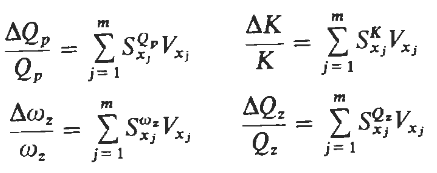
\includegraphics[scale=.5]{Secciones/Circ1/img/desvPorUnidad.png}
    \caption{Variabilidad en parametros por tolerancias de los componentes (Daryanani pag. 152).}
    \label{prop}
\end{figure}

Se realizo un script en PYTHON para calcular el cambio por unidad de $\omega_{p}$ y $bw_p$ con una tolerancia de los componentes del 10\% para ambas topologias analizadas.

\subsubsection{Realimentacion positiva (Sallen-Key)}

\noindent $>>$ \texttt{Siguiendo lo desarrollado en el Daryanani, y teniendo en cuenta que para este caso la tolerancia de todos los componentes es la misma:}

\begin{align*}
    \frac{\Delta\omega_{p}}{\omega_{p}} 
    = \sum_{i} S^{\omega_p}_{x_i} \frac{\Delta x_{i}}{x_{i}} 
    &= \frac{\Delta x}{x} (S^{\omega_{p}}_{R1}+S^{\omega_{p}}_{R2}+S^{\omega_{p}}_{R3}+S^{\omega_{p}}_{C1}+S^{\omega_{p}}_{C2}) \\ 
    &= 0.1 (S^{\omega_{p}}_{R1}+S^{\omega_{p}}_{R2}+S^{\omega_{p}}_{R3}+S^{\omega_{p}}_{C1}+S^{\omega_{p}}_{C2}) \\
    &= -0.2000 \\\\
    \frac{\Delta bw_{p}}{bw_{p}} 
    = \sum_{i} S^{bw_p}_{x_i} \frac{\Delta x_{i}}{x_{i}} 
    &= -0.2024
\end{align*}

Lo que significa que el el peor de los casos cuando los componentes varien un 10\% de su valor nominal, $\omega_{p}$ y $bw_{p}$ variaran un 20\% aproximadamente.

% ---------------------------------------------------
\subsubsection{Realimentacion negativa}

\noindent $>>$ \texttt{Siguiendo lo desarrollado en el Daryanani, y teniendo en cuenta que para este caso la tolerancia de todos los componentes es la misma:}

\begin{align*}
    \frac{\Delta\omega_{p}}{\omega_{p}} 
    = \sum_{i} S^{\omega_p}_{x_i} \frac{\Delta x_{i}}{x_{i}} 
    &= \frac{\Delta x}{x} (S^{\omega_{p}}_{R1}+S^{\omega_{p}}_{R2}+S^{\omega_{p}}_{R3}+S^{\omega_{p}}_{C1}+S^{\omega_{p}}_{C2}) \\ 
    &= 0.1 (S^{\omega_{p}}_{R1}+S^{\omega_{p}}_{R2}+S^{\omega_{p}}_{R3}+S^{\omega_{p}}_{C1}+S^{\omega_{p}}_{C2}) \\
    &= -0.2000 \\\\
    \frac{\Delta bw_{p}}{bw_{p}} 
    = \sum_{i} S^{bw_p}_{x_i} \frac{\Delta x_{i}}{x_{i}} 
    &= -0.2000
\end{align*}

Nuevamente se vio que en el peor de los casos cuando los componentes varien un 10\% de su valor nominal, $\omega_{p}$ y $bw_{p}$ variaran un 20\% aproximadamente.